\documentclass[conference]{IEEEtran}
\IEEEoverridecommandlockouts
\usepackage{stfloats} %针对双栏图 实现h t b p
\usepackage{makecell} %表格中一个单元格的文字换行
\usepackage{threeparttable} %表格注解
\usepackage{enumitem}  % item缩进
\usepackage{array}   % 表格内文字居中
\usepackage{booktabs}
%%%%%%%%%%%%%%%%%%%%%%%%%%%%%%%%%%%%%%%%%%%%%%%%%%%%%%%%%
%    Comments
%%%%%%%%%%%%%%%%%%%%%%%%%%%%%%%%%%%%%%%%%%%%%%%%%%%%%%%%%
\usepackage{verbatim}
%%%%%%%%%%%%%%%%%%%%%%%%%%%%%%%%%%%%%%%%%%%%%%%%%%%%%%%%%
%\usepackage[varg]{txfonts}
\usepackage{float}
\usepackage{bm}
\usepackage{eqparbox}
\usepackage{booktabs}
\usepackage{stmaryrd}
\usepackage{amssymb}
\usepackage{mathrsfs}
\usepackage{epsfig,graphics}
\usepackage{amsmath}
\usepackage{wasysym}
\usepackage{graphicx}
\usepackage{tabularx}
\usepackage{url}

%\usepackage{algpseudocode}
%\usepackage{appendix}

\usepackage{pgfplots}
\usepackage{pgfplotstable}
\usepackage{pgfplots} % used for showing all the figure
\pgfplotsset{
	compat=1.5
}

%\usepackage{cite}
\usepackage{amsfonts}

%�㷨����
\usepackage{algorithm}
%\usepackage[ruled]{algorithm2e}
\usepackage{algorithmicx}
\usepackage{algpseudocode}  %����
\usepackage{textcomp}  %����\textacutedbl �İ�,���׵�����
%\usepackage{authblk} %���߷�ʽ�� ��Ҫ�õİ���
\usepackage{xcolor}
%����ĺϲ� �кϲ�
\usepackage{multirow}
%������Ҽӵ�����ע�͵�
%\usepackage{comment}


\def\BibTeX{{\rm B\kern-.05em{\sc i\kern-.025em b}\kern-.08em
    T\kern-.1667em\lower.7ex\hbox{E}\kern-.125emX}}


\usepgfplotslibrary{groupplots}
%\usepackage[ngerman]{babel}
%%%%%%%%%%%%%%%%%%%%%%%%%%%%%%%%%%%%%%%%%%%%%%%%%%%%%%%%%
%    Algorithm
%%%%%%%%%%%%%%%%%%%%%%%%%%%%%%%%%%%%%%%%%%%%%%%%%%%%%%%%%
%\usepackage[]{algorithm2e}
%\usepackage{algorithmic}
\usepackage{algorithm}
\usepackage{multicol}
\usepackage{algpseudocode}
%%%%%%%%%%%%%%%%%%%%%%%%%%%%%%%%%%%%%%%%%%%%%%%%%%%%%%%%%


\newcommand{\Real}{{\mathbb R}}
\newcommand{\Inh}[2]{\mathsf{Inh}\mathsf{(#1, #2)}}
\newcommand{\Cal}[2]{\mathsf{Cal}\mathsf{(#1, #2)}}
\newcommand{\Con}[2]{\mathsf{Con}\mathsf{(#1, #2)}}
\newcommand{\Cre}[2]{\mathsf{Cre}\mathsf{(#1, #2)}}
\newcommand{\Ref}[2]{\mathsf{Ref}\mathsf{(#1, #2)}}
\newcommand{\rand}{\wedge}
\newcommand{\ror}{\vee}
\newcommand{\rimply}{\Rightarrow}
\newcommand{\rr}{\rightarrow}
\newcommand{\nr}{\rightsquigarrow}
\newcommand{\rnot}{!}
\newcommand{\Instances}[1]{\mathsf{Inst}\mathsf{(#1)}}
\newcommand{\TypeOf}[1]{\mathsf{Type}\mathsf{(#1)}}
\newcommand{\AttrValue}[2]{\mathsf{AttrVal}\mathsf{(#1, #2)}}
\newcommand{\Value}[1]{\mathsf{Val}\mathsf{(#1)}}
\newcommand{\InitialValue}[1]{\mathsf{InitVal}\mathsf{(#1)}}
\newcommand{\Contains}[2]{\mathsf{Con}\mathsf{(#1, #2)}}
\newcommand{\patomic}{\mathsf{atomic}}
\newcommand{\pskip}{\mathsf{skip}}
\newcommand{\pmf}[1]{\mathsf{#1}}
\newcommand{\szihao}{\fontsize{1pt}{1pt}\selectfont}
\newcommand{\sfrac}{\szihao \dfrac}
\newcommand{\WI}[1]{\texttt{#1}}
\newcommand{\cname}[1]{{\small ${#1}$}}
%\newcommand{\tabincell}[2]{\begin{tabular}{@{}#1@{}}#2\end{tabular}}
\renewcommand{\algorithmicrequire}{\textbf{Input:}}  % Use Input in the format of Algorithm
\renewcommand{\algorithmicensure}{\textbf{Output:}} % Use Output in the format of Algorithm


% correct bad hyphenation here
\hyphenation{op-tical net-works semi-conduc-tor}
\usepackage[square, comma, sort&compress, numbers]{natbib}
\usepackage{color}
\definecolor{gray}{rgb}{0.4,0.4,0.4}
\definecolor{darkblue}{rgb}{0.0,0.0,0.6}
\definecolor{cyan}{rgb}{0.0,0.6,0.6}
\usepackage{epstopdf}

\usepackage[colorlinks,
            linkcolor=black,
            anchorcolor=black,
            citecolor=blue,
			urlcolor=black,
            bookmarks=true
            ]{hyperref}


\newcommand{\TODO}[2]{{\textcolor{blue}{#1}}$\to${\textcolor{red}{#2}}}
\newcommand{\SOLVED}[2]{#2}
\newcommand{\HIGHLIGHT}[1]{{\textcolor{red}{#1}}}



%%%%%%%%%%%%%%%%%%%%%%%%%%%%%%%%%%%%%%%%%%%%%%%%%%%%%%%%%%%%%%%%%
\newcommand{\lds}[4]{
$\bb{#1}\sfbe{
	#2
}~=~
	\lambda #3.
(
	#4
)$}



\newcommand{\sfbe}[1]{\llbracket~#1~\rrbracket}

\newcommand{\denotationalsemantics}[4]{
{\footnotesize$
\bb{#1}\llbracket
	#2
\rrbracket=~\{
	#3
		~\mid~
	#4
\}$}}
\newcommand{\ins}[1]{$\lfloor$#1$\rceil$}
\newcommand{\lr}{\longrightarrow}
\newcommand{\bb}[1]{{\mathbb{#1}}}
\newcommand{\sfb}[1]{\textlbrackdbl~#1~\textrbrackdbl}
\newcommand{\la}{\langle}

\newcommand{\ra}{\rangle}
\newcommand{\nit}{\noindent}
\newcommand{\fbv}{formula_{bv}}
\newcommand{\s}{\sigma}
\newcommand{\sip}{\sigma^\prime}

%%%%%%%%%%%%%%%%%%%%%%%%%%%%%%%%%%%%%%
\newcommand{\code}[1]{{\texttt{#1}}}
\newcommand{\address}[1]{{\textcolor{gray}{\texttt{#1}}}}
\newcommand{\haddress}[1]{{\textcolor{blue}{\texttt{#1}}}}
\newcommand{\hcode}[1]{{\textcolor{blue}{\texttt{#1}}}} 

\begin{document}

\title{HexGANFuzzer: A Deep Adversarial Networks based Industrial Control Protocol Fuzzing Framework from A Self-Attention Perspective \\}
%\author{ %Anonymous
\IEEEauthorblockN{
Zhihui Li\IEEEauthorrefmark{2},
Jiawen Xiong\IEEEauthorrefmark{2},
%Hui Zhao\IEEEauthorrefmark{1},
Jianqi Shi\IEEEauthorrefmark{2} and
Yanhong Huang\IEEEauthorrefmark{2}\IEEEauthorrefmark{3}
}
%\IEEEauthorblockA{\IEEEauthorrefmark{1}National Trusted Embedded Software Engineering Technology Research Center\\
%East China Normal University, Shanghai, China\\
%}
\IEEEauthorblockA{\IEEEauthorrefmark{3}Hardware/Software Co-Design Technology and Application Engineering Research Center, Shanghai, China\\
}
\IEEEauthorblockA{\IEEEauthorrefmark{2}Shanghai Key Laboratory of Trustworthy Computing, East China Normal University, Shanghai, China\\
Email:\{zhihui.li, jiawen.xiong\}@ntesec.ecnu.edu.cn}
%Email:\{zhihui.li, hui.zhao, jianqi.shi, yanhong.huang, jiawen.xiong \}@ntesec.ecnu.edu.cn}
} 
\author{Wanyou Lv$^{1}$ \and
	Bohao Wang$^{1}$ \and
	Jianqi Shi$^{2,*}$ \and
	Yanhong Huang$^{3}$ \and
	Zhihui Li$^{4}$ 
}

%\authorrunning{Short form of author list} % if too long for running head


%\date{Received: date / Accepted: date}
\date{2020/04/07}
% The correct dates will be entered by the editor

% Comment for arXiv
%\titlerunning{Journal of Intelligent Manufacturing}
%\authorrunning{Journal of Intelligent Manufacturing}

%\titlerunning{

\maketitle
%, and its importance to the ICS is self-evident.
 %test the multi-dimensional input effectively but also 
\begin{abstract}
The Industrial Control Protocol (ICP) is the cornerstone of the communication of the Industrial Control System (ICS). If the security of ICPs can be guaranteed, the security of ICSs can be guaranteed to a large extent. However, the industrial control environment applicable to ICPs has a strong diversity, which causes the meaning of the same parameter in different applications varies greatly. It is difficult for testers to formulate a series of universal security rules. Therefore, fuzz testing (fuzzing) has already become the main method of detecting vulnerabilities in ICPs. It is noticed that the process of fuzzing relies heavily on specifications of ICPs. And it will take a lot of time and manual engineering to analyze and understand specifications. In this paper, we propose a new simple and smart sequence generation neural network framework based on Improved Wasserstein GANs (WGAN-GP), called HexGANFuzzer, to solve problems. Moreover, we put forward a series of performance metrics to evaluate different models in the field of fuzzing. Compared with traditional methods, our framework can generate massive fake but plausible test protocol messages automatically in a short time without protocol specifications. Compared with other deep learning works for fuzzing, our framework can not only increase the probability of triggering vulnerabilities but also be more parallelizable and require significantly less time to train. We evaluate its performance by testing several typical ICPs, including MQTT and Modbus. Extensive experiments demonstrate significant improvements of HexGANFuzzer on test effectiveness and efficiency: the accuracy that test case packages are generated correctly is 86.08\% and 92.71\% in datasets of different data scales, F-measure reaches 82.08\% and 85.02\%, and the test effectiveness and efficiency are 8.03\% and 5.26\% higher than the WGAN-based model.

%correctly generates the format and message content of the test case package. 其准确率分别为86.08%、92.71%,,F-measure分别达到了82.08%和85.02%,测试有效性和效率比WGAN-based model分别高了8.03%,5.26%。   
%\textcolor[rgb]{1,0,0}{\#\#\#\#\#\#\#\#  Here can specify specific values.}
\end{abstract}

\begin{IEEEkeywords}
deep adversarial learning, self-attention, convolution neural networks, fuzz testing, industrial control protocol
\end{IEEEkeywords}

\section{Introduction}

With the arrival of Industry 4.0 and Internet+, some new trends in the development of manufacturing. Strategic plans have been put forward to build the next generation of manufacturing. These strategies intend to empower the industry through information technology, such as optimizing the processes, reducing the costs and increasing the efficiency, to unlock greater productivity. The ICS, as the basic component of the automated production of the national economy and the people's livelihood, is a key part of the national safe strategy. The interaction between the ICS and its network environment becomes more frequent. The system is facing increasing external security threats. When applying the ICP into actual production, it is necessary to discover potential protocol vulnerabilities in time and prevent them in advance. 

Currently, applying traditional fuzz testing techniques to detect loopholes in ICPs is an effective method. However, there are some limitations to applying the techniques: (i) High demand for the testers. The tester is required to design appropriate test cases according to the communication protocol specification running in the system. (ii) Long test cycle. The entire testing process will last a long time. It is impossible to complete the test task efficiently when it is in urgent need. (iii) No versatility. Traditional methods design specific test cases based on specific test objectives, which is not universal.

Compared with traditional fuzzing works, deep learning methods for fuzzing bypass the process of building protocol specifications and protocol automata, reducing the workload and breaking the border of different protocols to achieve the generality. However, poor machine learning algorithms not only consume a lot of computing resources during the training of the model but also tend to generate a large number of error-formatted protocol message sequences after the training, resulting in normal crashes and error messages, which are quickly rejected by the server and prevent further testing.

In the process of fuzzing, there are a lot of crashes and error messages. But there is a challenge in distinguishing what of them are vulnerabilities and how to find real vulnerabilities from these crashes. In order to explore the balance between normal and abnormal exceptions, we propose a fuzzy test case generation methodology based on the ideal of deep adversarial learning in this paper. The contributions are summarized as follows:

\begin{itemize}
\item[(1)] We propose a methodology based on GAN to deal with fuzzy data generation, in which it can intelligently learn to generate testing data by itself. We apply Wasserstein distance\cite{arjovsky2017wasserstein}  to solve GAN's limitations for sequences of discrete, and introduce a penalty term to ensure the diversity of generated test case.
\item[(2)] On the premise of ensuring the lightweight of the model and saving computing resources, we introduce the self-attention mechanism which dispenses with recurrence and convolutions entirely and allows significantly more parallelization which requires significantly less time to train, makes it superior in quality of generating fake but plausible testing data in the process of model design.
\item[(3)] On top of the approach, we build a universal fuzzing framework based on improved SAGAN, called SAGANFuzzer, which can not only deal with the fuzzing of most ICPs but also show the superiority over other existing deep learning methods in theory and application. %\textcolor[rgb]{1,0,0}{Judge this part exist or not: Moreover, in the process of sampling, this paper introduces a series of anti-random strategies to improve the probability of anomalies throwing}
\item[(4)] Since there are no corresponding evaluation standards in fuzzing based on deep adversarial learning, we propose a series of metrics to evaluate the performance of our framework from the evaluation of the performance of the machine learning model and the evaluation of the vulnerability detection capability
\end{itemize}

To evaluate its performance, we apply it to test several ICPs. The experimental results show that our method has better performance than and can obtain excellent test results in different ICPs. In terms of test effectiveness and efficiency, the expected results are achieved.

The remainder of this paper is organized as follows. Section \uppercase\expandafter{\romannumeral2} discusses the related work. Section \uppercase\expandafter{\romannumeral3} details the optimized improved SAGAN algorithm and the entire methodology design. Section \uppercase\expandafter{\romannumeral4} presents the experiment and evaluation results. Section \uppercase\expandafter{\romannumeral5} concludes the paper and discusses some ideas about future work.

%\section{Preliminary}
In this section, we introduce some preliminary knowledge. First, the basis of LSTM, GAN and DCGAN is presented.  We then introduce the preliminary knowledge of ICPs and their common features. Lastly, we give an overview of fuzz testing and its application in finding ICPs' vulnerabilities.

\subsection{Long Short-Term memory}
Hochreiter and Schmidhuber (1997) first proposed LSTM to overcome the gradient vanishing problem of RNN (Recurrent Neural Networks). It is a special RNN that introduces an adaptive gating mechanism which can decides the degree to keep the previous state and avoid the problem of long-tern dependencies. Given a sequence $S = {x1, x2, …, xl}$, where $l$ is the length of input text, LSTM processes it word by word. At time-step $t$, the memory $c_{t}$ and the hidden state $h_{t}$ are updated with the following equations:
\begin{equation}
\left[ \begin{array}{c}
\Gamma _u^{ < t > }\\
\Gamma _f^{ < t > }\\
\Gamma _o^{ < t > }\\
{{\hat c}_t}
\end{array} \right] = \left[ \begin{array}{c}
\sigma \\
\sigma \\
\sigma \\
\tanh 
\end{array} \right]W \cdot \left[ {{h_{t - 1}},{x_t}} \right]
\end{equation}
\begin{equation}
{c_t} = \Gamma _f^{ < t > } \odot {c_{t - 1}} + \Gamma _u^{ < t > } \odot {\hat c_t}
\end{equation}
\begin{equation}
{h_t} = \Gamma _o^{ < t > } \odot \tanh ({c_t})
\end{equation}
where $x_{t}$ is the input at the current time-step, $\Gamma _u$, $\Gamma _f$ and $\Gamma _o$ is the update gate activation, forget gate activation and output gate activation respectively, $\hat{c}$ is the current cell state, $\sigma$ denotes the logistic sigmoid function and $\odot$ denotes element-wise multiplication.

\subsection{Generative Adversarial Networks}
Generative Adversarial Networks, proposed by Goodfellow and others, is a promising framework to guide the training of generative models. Specifically, in GAN, a discriminative network $D$ (discriminator) learns to distinguish whether a given data instance is real or not, and a generative network $G$ (generator) learns to confuse discriminator by generating fake but plausible data. 

In this adversarial network framework, the goal of the training generation model is to obtain a probability distribution of $P_z$, which approximates the distribution $P_x$ of the real data $x$. In order to achieve this goal, a known distribution (such as Gaussian distribution, uniform distribution) is used to sample and get the ``noise data " (represented by $z$) in the first place. Then, these ``noise data" are input into the generation model, and the training of the generation model is carried out. After the training of the generator is finished, simulated data is output. 

In this study, we utilize this feature to generate simulated sequence messages. Notably, when applying deep adversarial learning to fuzz testing ICPs, we expect the generated data to have a correct message format but with various message content so that the code coverage and testing depth can be guaranteed. 

%\begin{figure}[htbp]
%\centering
%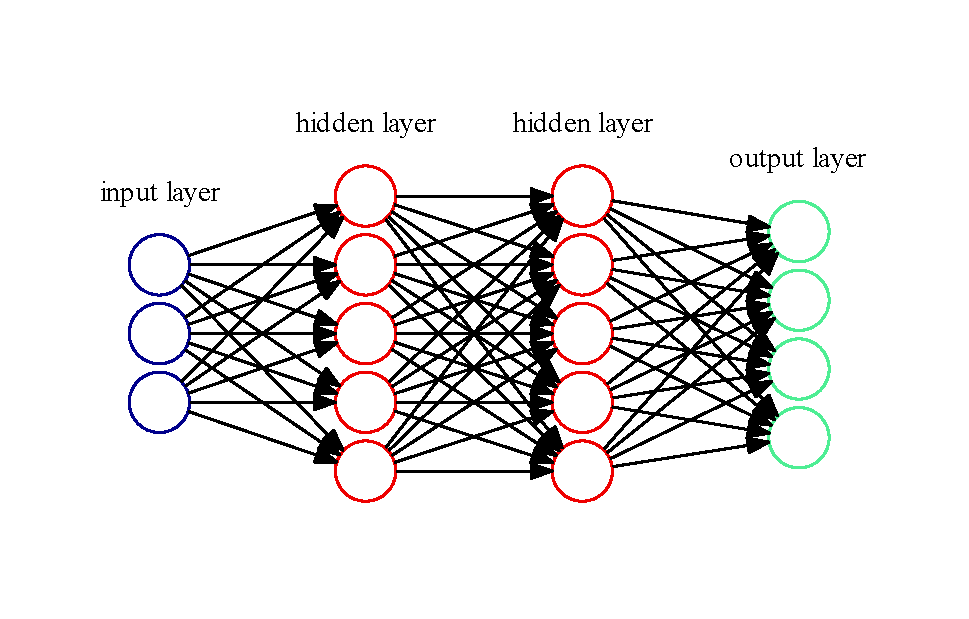
\includegraphics[scale=0.4]{FIGURE/FIGURE_NNSTRUCT.pdf}
%\caption{Multilayer Perceptron}
%\label{FIGURE_NNSTRUCT}
%\end{figure}

\subsection{Deep Convolution Generative Adversarial Networks}
Prior to introducing DCGAN, it is necessary to briefly introduce CNNs (Convolution Neural Networks), which have recently enjoyed great success in image and video recognition. Its success is mainly due to the large public image repositories, such as ImageNet, and high-performance computing systems, such as GPUs (Graphics Processing Units) or large-scale distributed clusters. Because the pooling layer has no weights, no parameters and only a few hyperparameters, one convention comprises one convolutional layer part and one pooling layer part in general. A typical CNN consists of many layers, including the input layer, conventions, the fully-connected layer, the output layer, etc.

Recently, NLP communities pay more and more attention to CNN and have achieved favorable results in various text classification tasks \cite{kim2014convolutional,zhang2015character}. Different from RNNs accomplished in time-related problems, CNN is good at learning spatial structure features. Actually, most ICPs’ messages have the following features: concise format, limited length and compact structure. This makes CNN a better way to solve this kind of problem \cite{kim2014convolutional}. After proper preprocessing via Bi-LSTM which adds the location feature in the input, each filter in CNN can be regarded as a detector that detects whether a functional unit in the data frame is correct \cite{adel2016exploring}, which is conducive to grasping the format features of the sequence data in ICS.  Hence in this study, CNN serves as the generator and the discriminator in DCGAN accordingly.

DCGAN is proposed by Alec Radford et al. \cite{radford2015unsupervised} to bridge the gap between the success of CNNs for supervised learning and unsupervised learning. They extend GAN to the CNN domain and invent a structure called deep convolution generative adversarial networks (DCGAN) that have certain architectural constraints. This innovation combines the advantages of CNN in processing multidimensional features and the idea of deep adversarial learning. Due to the constraints, DCGAN largely overcomes the problem of unstable training of GANs, such as non-convergence, vanishing gradient and mode collapse.  These constraints are listed in Table \uppercase\expandafter{\romannumeral1}. We designed our model architecture based on the constraints.


\begin{table}[htbp]
\caption{Architecture guidelines for stable Deep Convolutional Generative Adversarial Networks}
\label{table_example}
\centering
\begin{tabular}{|c|c|}
\hline
\bfseries \# & \bfseries Architecture constraints\\
\hline
1 & \multicolumn{1}{m{7cm}|}{Replace any pooling layers with strided convolutions (discriminator) and fractional-strided convolutions (generator).}\\
\hline
2 & \multicolumn{1}{m{7cm}|}{Use batch normal in both the generator and the discriminator.} \\
\hline
3 & \multicolumn{1}{m{7cm}|}{Remove fully connected hidden layers for deeper architectures.} \\
\hline
4 & \multicolumn{1}{m{7cm}|}{Use ReLU activation in the generator for all layers except for the output, which uses Tanh.}\\
\hline
5 & \multicolumn{1}{m{7cm}|}{Use LeakyReLU activation in the discriminator for all layers.}\\
\hline
\end{tabular}
\end{table}


\subsection{Industrial Control Protocols}
ICPs refers to the communication protocol deployed in ICSs. As a class of systems, ICS has its characteristics, such as requiring high real-time performance and just providing several specific functions. Correspondingly, ICP's message format tends to be concise. ICS consist of master stations and slave stations. The data transmission and operation control between them are realized through the ICP in it. Currently, various ICPs operate in a wide variety of ICSs around the world. Therefore, it is important to maintain ICPs' safety and security. Except for the popular ICPs, Some ICPs are modified from the existing protocols or solely designed. These ICPs may have no clear specifications. Thus, the manual-based fuzz testing method will suffer from this.

\subsection{Fuzz Testing}
Fuzz testing is a quick and cost-effective method for finding severe security defects in software. Traditionally, fuzz testing tools apply random mutations to well-formed inputs of a program and test the resulting values. Besides, fuzzing is a brute force vulnerability method, in which it uses a large amount of malicious input to have stress tests on the target. As industrial control networks become more and more interconnected, flaws in the implementations of ICP could allow a malicious party to attack vulnerable systems remotely over the internet. To avoid this, we use fuzzing to discover the flaws in advance. The workflow is shown in Fig.  \ref{FigFuzzingFlow}.
\begin{figure}[htbp]
	\centering
	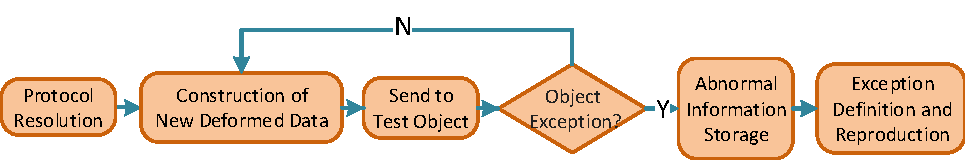
\includegraphics[width=3.5in]{FIGURE_LV/FigFuzzingFlow.pdf}
	\caption{General workflow of fuzzing test}
	\label{FigFuzzingFlow}
\end{figure}


%@article{gorbunov2010autofuzz,
%	title={Autofuzz: Automated network protocol fuzzing framework},
%	author={Gorbunov, Serge and Rosenbloom, Arnold},
%	journal={IJCSNS},
%	volume={10},
%	number={8},
%	pages={239},
%	year={2010}
%}
\section{Related Works}

Fuzzing is a stress test by inputting a large number of unexpected abnormal inputs into the test target so as to trigger abnormal behavior of the target system \cite{kaschner2009automatic}. %, and find the exploitable vulnerabilities in the system. The prototype of fuzzing is Random Testing \cite{kaschner2009automatic}. 
Duran and Ntafos are pioneers in this field \cite{duran1984evaluation}. %In the early research, arbitrary input was used to test computer programs and good results were achieved. The concept of fuzzing was formally proposed by Miller et al. \cite{miller1990empirical} in 1990 and was initially applied to the testing of Unix programs. 
Since then, a variety of different techniques have been proposed to improve the efficiency of fuzzing. These techniques include static analysis \cite{sparks2007automated} and  %\cite{kinder2009abstract} 
dynamic analysis  %\cite{hoschele2016mining}
\cite{bastani2017synthesizing}. %\cite{kifetew2017generating}
Because of these methods, fuzzing has been studied in the network protocol testing field to enhance the reliability of the computer network %\cite{aitel2002introduction} \cite{amini2010sulley} %\cite{gorbunov2010autofuzz} 
%\cite{eddington2011peach} \cite{tsankov2012secfuzz}
 \cite{chen2018iotfuzzer} \cite{martin2019catalogue}. 
And some of these works are for ICPs and have made a certain contribution to the improvement of the safety and security of ICPs. %sssGreg Banks et al. proposed a fuzzy test tool called SNOOZE \cite{banks2006snooze} for stateful network protocols. 
%Devarajan et al. \cite{devarajan2007unraveling} released a fuzzy test module based on the Sully tool for Modbus, DNP3 and other industrial control protocols. Voyiatzis et al. \cite{voyiatzis2015modbus} designed a Modbus-TCP fuzzy test tool called MTF which builds the test model by Modbus official instructions.
%Boofuzz \cite{pereyda2017boofuzz}, proposed by Pereyda et al., aims not only for numerous bug fixes but also for extensibility in the field of network protocol fuzzing.

However, fuzzing for ICPs still faces many challenges, such as how to mutate seed inputs, how to increase code coverage, and how to effectively bypass verification \cite{li2018fuzzing}.
With the advancement of machine learning in the field of cybersecurity, it has also been adopted by many studies for vulnerability detection %\cite{grieco2016toward} 
\cite{wu2017vulnerability} \cite{xia2018remote} , including the applications in fuzzing \cite{godefroid2017learn} %\cite{rajpal2017not} \cite{wang2017skyfire} \cite{she2019neuzz}
\cite{chen2018systematic}. ICPs have many features in common such as short-data frames and no encryption. They are designed to satisfy the real-time requirements of ICSs. As expected, some studies have incorporated fuzzing algorithms of ICPs based on deep learning into the fuzzing process of ICPs \cite{li2019intelligent}. %\cite{hu2018ganfuzz} %Machine learning technology is introduced into fuzzing to provide a new idea for solving the bottleneck problems of the traditional fuzzing technology and also makes the fuzzing technology intelligent. With the explosive growth of machine learning research, using machine learning for fuzzing will become one of the critical points in the development of vulnerability detection technology.
 These efforts all contribute to fuzzing based on deep learning.

There are still some limitations of these aforementioned fuzzing algorithms based on deep learning, such as unbalanced training samples, lack of feature classification ability of industrial communication behaviors, and difficult to extract the characteristics related to vulnerabilities. We integrate the characteristics of self-attention and GAN to propose a deep convolution generative adversarial networks based fuzzing methodology and design an automated and intelligent fuzzing framework based on it, named HexGANFuzzer. %And with using Wasserstein distance and a gradient penalty (WGAN-GP) \cite{gulrajani2017improved}, our framework can not only solve the problem of poor performance for discrete data but also ensure the diversity of generated test cases.

%Self-attention \cite{vaswani2017attention}, an attention mechanism relating to different positions of a single sequence, allows attention-driven, long-range dependency modeling for generation tasks. GAN, with a discriminative network D (discriminator) which learns to distinguish the reality of a
%given data instance, and a generative network G (generator) which learns to confuse discriminator, can generate fake but plausible data via an adversarial learning process. 


\section{HexGANFuzzer Framework}
In this section, we first acquire a large number of communication data from the ICS to be tested and then preprocess the data as the training data of the deep adversarial learning model established. Secondly, a generative model and a discriminant model are designed to generate the adversarial network, and a specific model is obtained by training and retraining the model with the acquired data. Finally, a series of performance metrics are put forward to evaluate our model.


\subsection{Preprocessing of ICP Message Frames}
In order to get diverse test cases, reach high code coverage and desirable fuzzing results, data preprocessing is a necessary part. There are two steps in preprocessing: \textbf{Message Frame Clustering} and \textbf{Data Conversion}.

\subsubsection{\textbf{Message Frame Clustering}}
After message frames collection, there are many different length message frames of the ICP. We adopted the Length Clustering method to preprocess the data frames. It is noted that most message frames with the same length share the same frame type. First, we gather the data frames which have the same length. In order not to get too many groups of data frames, groups whose quantity is less than a threshold (e.g. 5000) will be moved to the longer adjacent group, while group contains more data than the threshold are left unchanged. In such a way, there may be message frames with different lengths in one group. After clustering, the max length of message frames of every group will be the standard length and message frames whose length is less than max length will be added special token `u' at the end of them.

\subsubsection{\textbf{Data Conversion}}
The raw data frame of most protocols is hexadecimal, which can not be fed into the model directly. So after clustering, the hexadecimal data frames will be mapped into the digital vectors. The vocabulary we use is as followed:
\begin{equation}
\textit{\textbf{0 1 2 3 4 5 6 7 8 9 a b c d e f u}}
\end{equation}
The size of the vocabulary is 17, there are ten digits and seven hexadecimal characters according to the hexadecimal message frames and the supplement token `u'.
Based on the vocabulary, message frames $x \in R^{seq\_size \times 1}$ were converted into one hot vector $X \in R^{seq\_size \times 17}$(seq\_size is the max length of the current group), and one-hot vectors of real message frame will be the input of the critic.

\begin{figure}[htbp]   %  插入一栏图片
	\centering 
	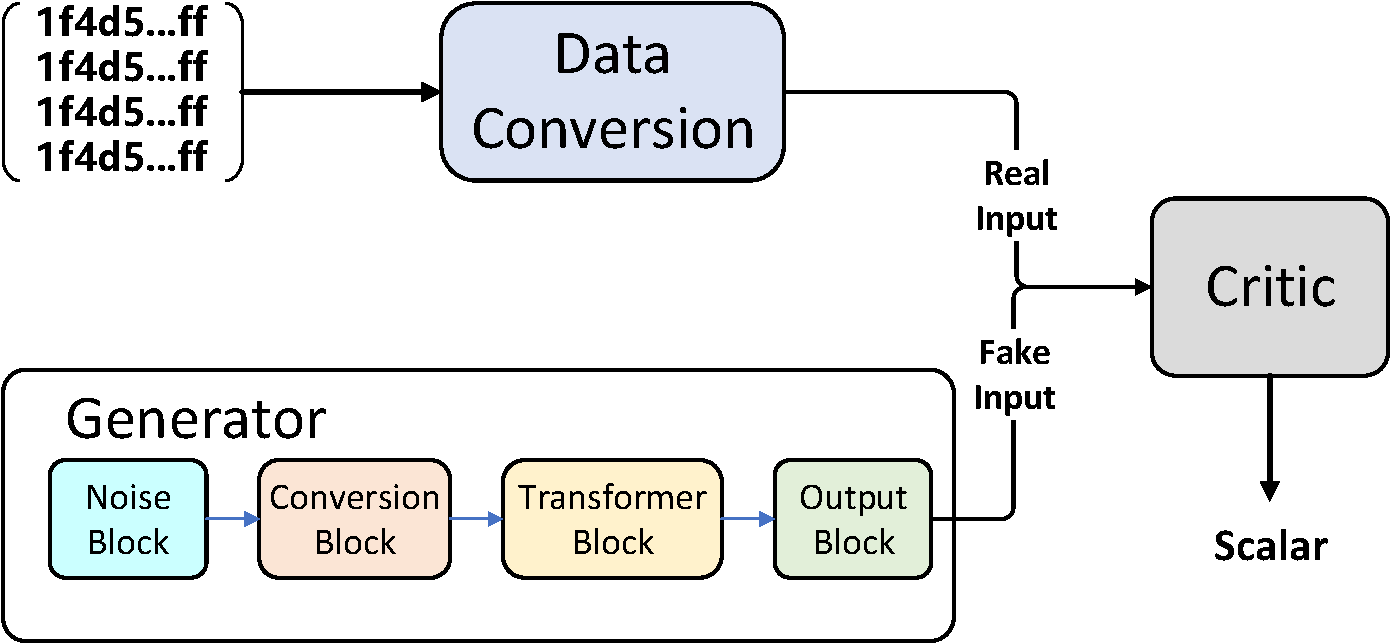
\includegraphics[width=3.5in]{FigHexGANFuzzer_model.pdf}
	\caption{The architecture of HexGANFuzzer}
	\label{FigHexGANFuzzer_model}
\end{figure}
\subsection{Model Design} 
\label{sec:model_design} 
In this part, we describe our test case generation model in detail. As Fig. \ref{FigHexGANFuzzer_model} shows, our model consists of a generator and a critic, which is the same as a WGAN model. The generator is born to generate the fake message frames and the critic will evaluate the Wasserstein distance. The Wasserstein distance is the minimum cost of transporting mass in converting the data distribution $q$ to the data distribution $p$. During the training, the Wasserstein distance between real message frame distribution and fake message frame distribution will be shortened and our model grasps the knowledge of the protocol grammar.

\begin{figure}[htbp]   %  插入一栏图片
	\centering 
	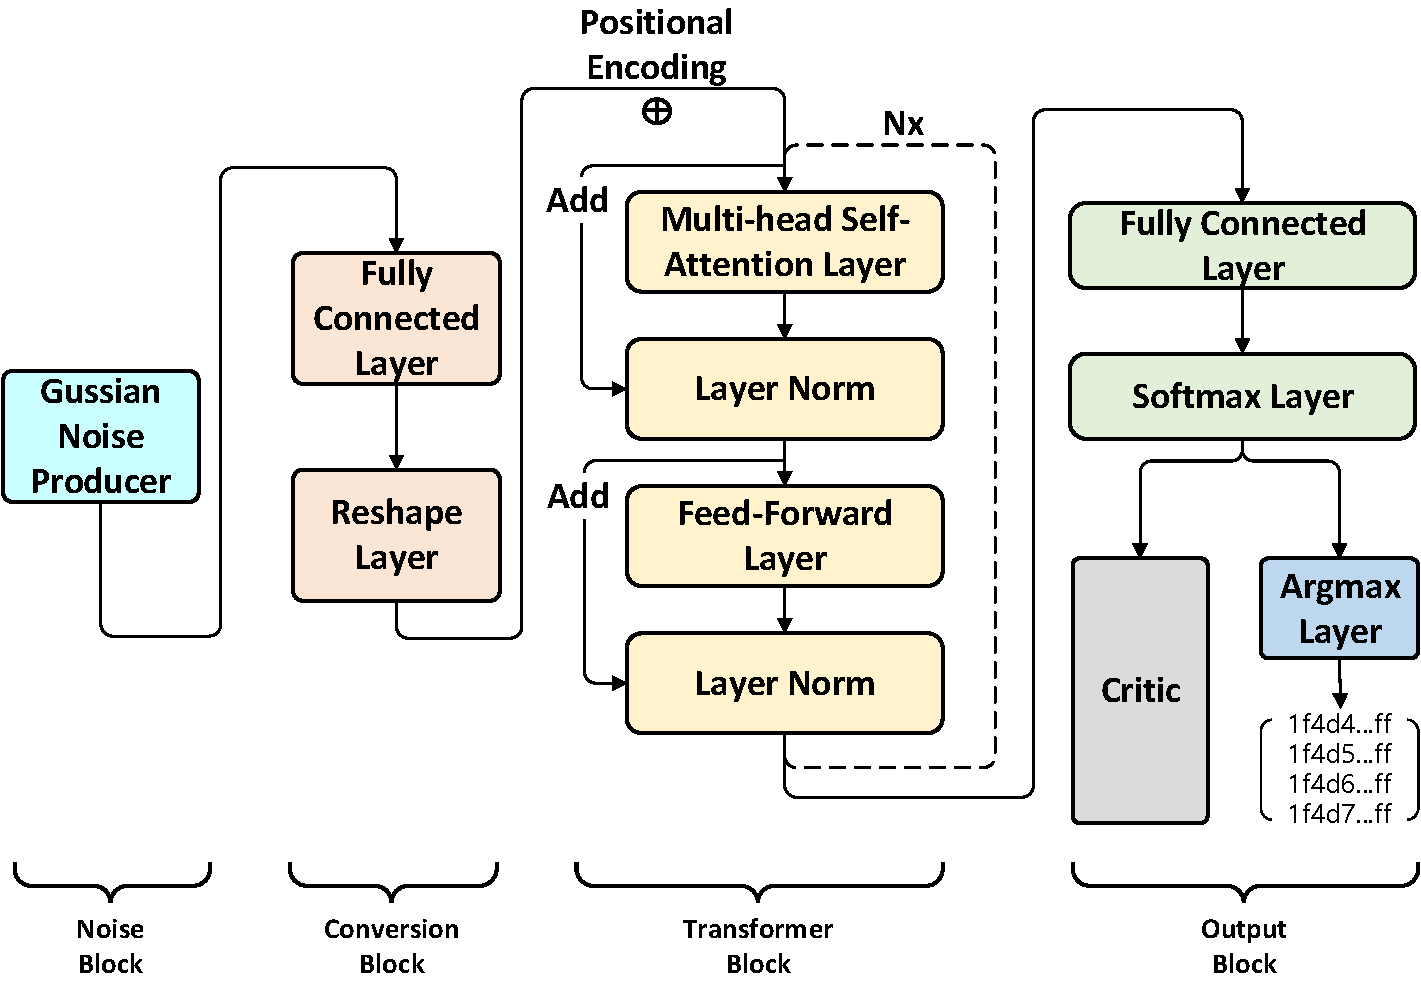
\includegraphics[width=3.5in]{FigHexGANFuzzer_Generator.pdf}
	\caption{Generator Network}
	\label{FigHexGANFuzzer_Generator}
\end{figure}
\subsubsection{\textbf{Generator}}

%总体描述,分为四个部分,四个部分里面分别是什么,简单介绍作用
The structure of the generator is as followed in Fig. \ref{FigHexGANFuzzer_Generator}. There are four parts, noise block, conversion block, transformer block, and output block. In order to generate different message frame data every time, the noise block will output some random noise data $z \in \mathbb{R}^{1 \times zd}$ where $zd$ is the initial dimension of the noise. And it is a common practice to set the noise data to Gaussian distributed noise. 

The conversion block contains a fully connected layer and a reshape layer. This block will convert the noise data $z$ into Noise Conversion Representation (NCR) $\tilde{z} \in \mathbb{R}^{ss \times dm}$ where $ss$ is the max sequence length of the current group and $dm$ is the number of feature dimension.

The transformer block contains a positional encoding layer and a sub-block. The sub-block is the same as the encoder part of the Transformer \cite{vaswani2017attention}. It is formed by a multi-head self-attention layer and a feed-forward layer. Besides, there is a residual connection around each of the two layers, followed by layer normalization. And the input and output of the transformer block are the same, so this part can repeat as many times as we want.

The output block is a fully connected layer and a softmax layer. After the conversion block and the transformer block, the generator will not output the message frame data directly, instead, it outputs a probability vector $\tilde{x} \in \mathbb{R}^{ss \times vs}$. Where $vs$ is the size of vocabulary, which is $17$ in our situation. The probability vector is an intermediate result which is used to feed to the critic. To obtain the message frame which can be sent, the probability vector will be applied $argmax$ function and be translated into hexadecimal data according to the vocabulary mentioned before.

The sequence information is normally one-dimensional vector, but during the computation in the NLP model, the sequence information is represented by two-dimensional vectors including word embedding or one-hot vector for the sake of a better representation of the sequence. 
For example, the input words of \cite{vaswani2017attention} are converted into word embedding. In our model, the two-dimensional vector is NCR. 
The reason we use NCR is that the output of the noise block is a random noise vector, which is hard to get the corresponding word embedding. In the NLP tasks, discrete data is usually regarded as the result of continuous sampling from the categorical distribution. If we force to find the word embedding with some tricks, it may cause the whole procedure non-derivable, which will make the backpropagation algorithm unavailable. 
The solution of most GAN text generation model is using the one-hot vector to replace the word embedding in the model. In this paper, our solution is NCR. Define the fully connected layer as $f$, processed by fully connected layer, ReLU activation and reshape operation, noise data $z$ will become $\tilde{z} = Reshape(f(z))$ and $ \tilde{z} \in \mathbb{R}^{ss \times {dm}}$. And it is the input of the transformer block.
NCR looks like word embedding, but it is fake. NCR maps the one-dimension noise vector to high dimensional space information. Compared with the one-hot vector, NCR can cover more information of high dimension space.


The transformer block is a feature extractor. Compared with the commonly used feature extractor, Recurrent Neural Network (RNN), the transformer block is better in semantic feature extraction and long-range feature extraction. Moreover, the self-attention layer in the transformer block supports parallel training, which can accelerate the training process.
The loss function of the generator is 
\begin{equation}
L_{g} = - \mathop{\mathbb{E}}\limits_{\tilde{x}\sim\mathbb{P}_{g}}\left [ D(\tilde{x}) \right ] 
\end{equation}
where D is a 1-Lipschitz function, $\tilde{x} \in \mathbb{R}^{ss \times vs}$ is the output of the generator, $\mathbb{P}_g$ is the model distribution implicitly defined by $\tilde{x}=G(z)$, and $z$ is the noise data.

\begin{figure}[htbp]   %  插入一栏图片
	\centering 
	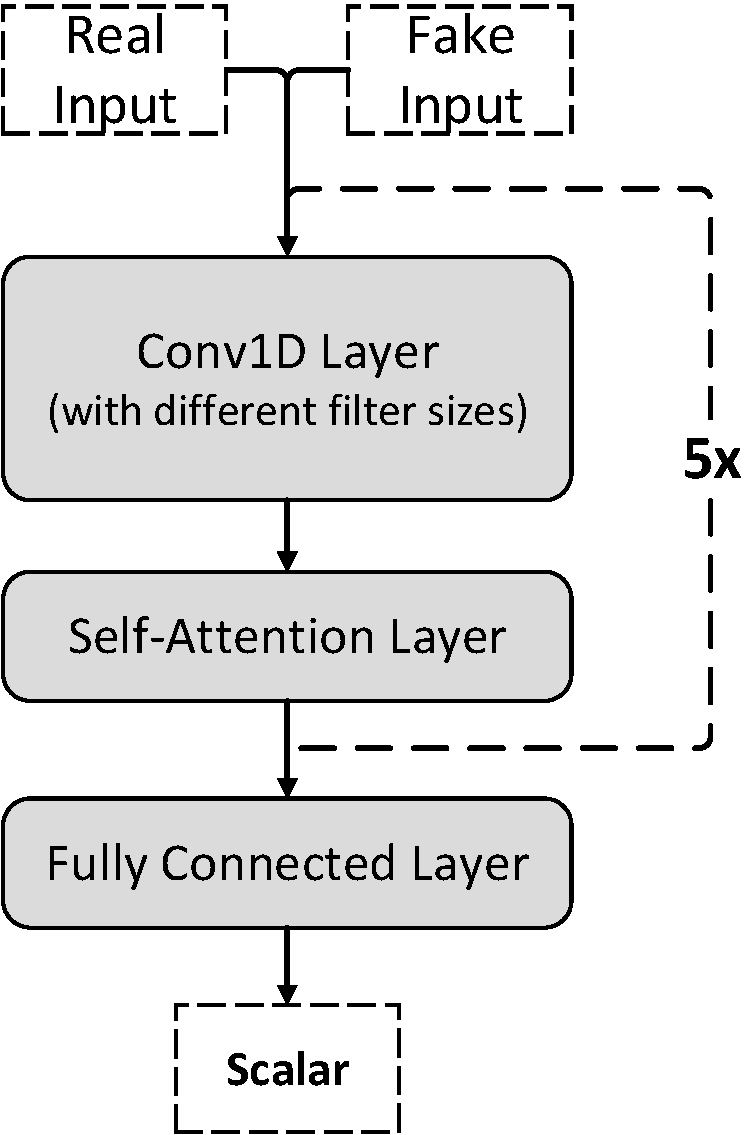
\includegraphics[width=1.5in]{FigHexGANFuzzer_Critic.pdf}
	\caption{Generator Network}
	\label{FigHexGANFuzzer_Critic}
\end{figure}
\subsubsection{\textbf{Critic}}
It looks like discriminator in normal GAN model, but it is not a classifier, we call it critic here, which is the same as WGAN \cite{arjovsky2017wasserstein}. The structure of the critic is as Fig. \ref{FigHexGANFuzzer_Critic} shows. The critic includes five conv1d layers, five self-attention layers, and one fully connected layer. For the critic, there are two types of inputs. One is the one-hot vector from the real message frames, and another is the output of the generator which represents the fake message frames. 
The second dimension of the output of the generator means the probability of each word in the vocabulary, and one-hot vector can also be understood as a special case of it, that is, the probability of one word is 1 and the probability of other words is 0. 

It is noted that the first conv1d layer changes the second dimension of inputs from the probability of word to the feature representation, which is the same as the dimension of NCR. And other conv1d layers keep the second dimension as $dm$. Every conv1d layer followed by a self-attention layer but the kernel size of conv1d is not the same. The kernel size of $i$th conv1d layer $ks_i = i$ where $i \in \{1,2,3,4,5\}$. 

Protocols have message headers, which specify the content of the message body in the message frame. More simply, the front part of the message frame affects the back part. It is hard to distinguish the boundary of two parts without the knowledge of the protocol grammar. If the model has learned which part is the message header, it can pay more attention to the message header part.
Due to different protocols have different lengths of the message header, the conv1d layer with different kernel size can capture the information better.
As for the content in the message header, several flags in the message header affect different parts of the content in the message body. self-attention layers can capture how flags in the message header affect the part of the message body.

The self-attention layer considers the attention weight of every position of the input and is good at learning long-range dependencies. With the boundary information leaned by conv1d layers, self-attention layers will pay more attention to the correlation between the content in the message header and body. After repeated self-attention and conv1d layers five times, the fully connected layer will output a scalar score. 
The loss of the critic is:
\begin{equation}
L_{c} = \mathop{\mathbb{E}}\limits_{\tilde{x}\sim\mathbb{P}_{g}}\left [ D(\tilde{x}) \right ] 
- \mathop{\mathbb{E}}\limits_{x\sim\mathbb{P}_{r}}\left [ D(x) \right ] 
+ \lambda\mathop{\mathbb{E}}\limits_{\hat{x}\sim\mathbb{P}_{\hat{x}}}\left [ ( \left \| \triangledown_{\hat{x}}D( \hat{x}) \right \|_{2} - 1 )^{2} \right ]
\end{equation}
where $\mathbb{P}_{\tilde{x}}$ define sampling uniformly along straight lines between pairs of points sampled from the real data distribution $\mathbb{P}_{r}$ and the generator distribution $\mathbb{P}_{g}$. 
In order to satisfy the 1-Lipschitz constraint, the solution of the WGAN-GP model was adopted. 
We use gradient penalty instead of the weight clipping to enforce the 1-Lipschitz constraint. 
It leads to a more stable training process and the model is easier to train.

\subsubsection{\textbf{Training strategy}}
Once the model design is completed, we begin to train our model. Under normal circumstances, the training of the GAN is adversarial, which means the generator and discriminator (critic) should be on the same level. If the imbalance is too serious, another one will learn nothing. And this is the reason why the GAN model is difficult to train and the training is unstable.
Due to the properties of the Wasserstein distance, we can train the critic better first and then narrow the Wasserstein distance between fake message frame distribution and real message frame distribution, which is the process of improving generator. In every epoch, we train generator once and then train the critic $c\_iters$ ($5$ in our model) times. Adam Optimizer was used both in the generator and the critic. In order to judge the convergence of the model, the following equation, which is the approximate value of the Wasserstein distance, is an indicator. If the value of the equation trends to be stable, we consider the model is convergent.
\begin{equation}
W\_distance = 
\mathop{\mathbb{E}}\limits_{x\sim\mathbb{P}_{r}}\left [ D(x) \right ] 
- \mathop{\mathbb{E}}\limits_{\tilde{x}\sim\mathbb{P}_{g}}\left [ D(\tilde{x}) \right ] 
\end{equation}
Though the model wants to generate the fake message frames that share high similarity to the real message frames, the ulmate goal is to achieve effective fuzzing results and identify as many bugs as possible. In order to obtain the desired results, there should be some differences between the real data and the fake data. So we not only save the final version of the model, which is convergent, but also the intermediate generator model. The model was saved every 10 training epoch deliberately. In such a training strategy, the goal of the high code coverage and deeper testing depth can be achieved.


\subsection{Performance Metrics}
Some quantitative criteria \cite{heusel2017gans} \cite{karras2017progressive} \cite{lucic2018gans} have emerged recently for evaluating the performance of GAN on image generation. However, there is no corresponding evaluation metrics in fuzzing based on deep adversarial learning, and the lack of these indicators includes two aspects: the evaluation of the performance of the machine learning model \cite{karras2017progressive} \cite{lucic2018gans} in the field of fuzzing based on deep learning \cite{shmelkov2018good} and the evaluation of the vulnerability detection capability. Therefore, in accordance with our research purpose and specific situation, the following evaluation metrics are proposed in this study.

%represents the percentage of correctly generating characters about function codes in generated test case sequences versus function codes in real test case packages
\subsubsection{\textbf{F-measure}}
In order to further demonstrate the performance of our model in this paper, we compare the performance of different models on test data generation of ICPs with several indexs such as \textit{Sensitivity}, \textit{Specificity}, \textit{Accuracy} and \textit{F-measure}.  Among them, Sensitivity represents the percentage of function codes for correctly generated test case packages versus function codes for real test case packages, Specificity means to the percentage of non-essential hexadecimal characters for correctly generated test case packages versus non-essential hexadecimal characters for real test case packages, and Accuracy is the percentage of the entire test case that correctly generates the format and message content of the test case package. The specific formula is as follows:
\begin{equation}
Accuracy = \frac{{TP + TN}}{{TP + FN + TN + FP}}
\end{equation}
\begin{equation}
Sensitivity = \frac{{TP}}{{TP + FN}}
\end{equation}
\begin{equation}
Specificity = \frac{{TN}}{{TN + FP}}
\end{equation}
\begin{equation}
Precision = \frac{{TP}}{{TP + FP}}
\end{equation}
\begin{equation}
Recall = \frac{{TP}}{{TP + FN}}
\end{equation}
\begin{equation}
\begin{array}{l}
F - measure =\displaystyle{2 \times Precision \times}  \\
\\{\kern 1pt} {\kern 1pt} {\kern 1pt} {\kern 1pt} {\kern 1pt} {\kern 1pt} {\kern 1pt} {\kern 1pt} {\kern 1pt} {\kern 1pt} {\kern 1pt} {\kern 1pt} {\kern 1pt} {\kern 1pt} {\kern 1pt} {\kern 1pt} {\kern 1pt} {\kern 1pt} {\kern 1pt} {\kern 1pt} {\kern 1pt} {\kern 1pt} {\kern 1pt} {\kern 1pt} {\kern 1pt} {\kern 1pt} {\kern 1pt} {\kern 1pt} {\kern 1pt} {\kern 1pt} {\kern 1pt} {\kern 1pt} {\kern 1pt} {\kern 1pt} {\kern 1pt} {\kern 1pt} {\kern 1pt} {\kern 1pt} {\kern 1pt} {\kern 1pt} {\kern 1pt} {\kern 1pt} {\kern 1pt} {\kern 1pt} {\kern 1pt} {\kern 1pt} {\kern 1pt} {\kern 1pt} {\kern 1pt} {\kern 1pt} {\kern 1pt} {\kern 1pt} {\kern 1pt} {\kern 1pt} {\kern 1pt} {\kern 1pt} {\kern 1pt} {\kern 1pt} {\kern 1pt} \displaystyle\frac{{Recall}}{{Precision + Recall}}
\end{array}
\end{equation}
wherein, TP is the number of correctly generated hexadecimal characters that constitute the function codes of ICPs' packages, TN is the number of correctly generated other non-essential hexadecimal characters including message content of ICPs' packages, FP is the number of hexadecimal characters  generated by error that constitute the function codes of ICPs' packages, and FN is the number of generated by error other non-essential hexadecimal characters including message content of ICPs' packages.

\subsubsection{\textbf{Effectiveness of Vulnerability Detection (EVD)}}
EVD refers to the ability to trigger anomalies on basis of the test target accepting the test data. The effectiveness of fuzzing depends predominantly on the testing depth and high code coverage. Therefore, we propose the effectiveness evaluation metric EVD for fuzzing models from the above two aspects.
%  The effectiveness evaluation of the fuzzing methods can be divided into two aspects: testing depth and code coverage.

When the generated data can be accepted by the test target, it indicates that the generated data is similar to real data in terms of the format, embodying that the model has the ability to learn the format of data frames from the real world. This phenomenon also reflects a certain depth of testing. But our ultimate goal is to trigger as many anomalies as possible to the ICS to find vulnerabilities, so two sub-metrics are taken into account when we finally calculate the testing depth for EVD: \textit{Acceptance Rate of Test Cases (ARTC)} and \textit{Ability of Vulnerability Detected (AVD)}:

\quad \textit{\textbf{a. ARTC.}} ARTC refers to the acceptance rate at which the generated test data is received by the test target when it is sent to the test target. The specific formula is as follows:
\begin{equation}
ARTC = \frac{{N_{accepted}}}{{N_{all}}} \times 100\%  
\end{equation}
where ${N_{accepted}}$ is the total number of test cases accepted and ${N_{all}}$ is the total number of test cases sent.

\quad \textit{\textbf{b. AVD.}} AVD refers to the ability of triggering anomalies for the test target when the generated test data is sent to the test target. We define AVD as follows:
\begin{equation}
AVD = \frac{{N_{anomalies}}}{{N_{all}}} \times 100\%  
\end{equation}
where ${N_{anomalies}}$ is the total number of test cases which trigger anomalies and ${N_{all}}$ is the total number of test cases sent.

\textit{\textbf{Diversity of Generated Cases (DGC)}} is a sub-metric proposed as the extent of code coverage for fuzzing in EVD. It refers to the ability to maintain the diversity of the generated data. The diversity-based approach is a useful test case selection criterion for code coverage \cite{hemmati2013achieving} \cite{mondal2015exploring}. Furthermore, more diverse generated test data frames are likely to cause more exceptions. And this indicator focuses on the number of message types in the generated data, see the following formula: 
\begin{equation}
DGC = \frac{{N_{gen\_categories}}}{{N_{all\_categories}}} \times 100\% 
\end{equation}
where $N_{gen\_categories}$ is the total number of message categories in the generated data frames, and $N_{all\_categories}$ is the total number of message categories in the training dataset.

In order to balance the different weights of sub-metrics on model effectiveness, dimensionless quantity method is applied to eliminate the influence of different scales between sub-metrics so that each sub-metric can be converted into a value that can be directly added or subtracted. We normalize aforementioned sub-metrics and add them up to get the comprehensive scores for EVD:
\begin{equation}
\begin{array}{l}
EVD=(\displaystyle\frac{{ART{C_i} - ART{C_{\min }}}}{{ART{C_{\max }} - ART{C_{\min }}}} + \frac{{VD{E_i} - VD{E_{\min }}}}{{VD{E_{\max }} - VD{{E}_{\min }}}}\\
\\{\kern 1pt} {\kern 1pt} {\kern 1pt} {\kern 1pt} {\kern 1pt} {\kern 1pt} {\kern 1pt} {\kern 1pt} {\kern 1pt} {\kern 1pt} {\kern 1pt} {\kern 1pt} {\kern 1pt} {\kern 1pt} {\kern 1pt} {\kern 1pt} {\kern 1pt} {\kern 1pt} {\kern 1pt} {\kern 1pt} {\kern 1pt} {\kern 1pt} {\kern 1pt} {\kern 1pt} {\kern 1pt} {\kern 1pt} {\kern 1pt} {\kern 1pt} {\kern 1pt} {\kern 1pt} {\kern 1pt} {\kern 1pt} {\kern 1pt} {\kern 1pt} {\kern 1pt} {\kern 1pt} {\kern 1pt} {\kern 1pt} {\kern 1pt} {\kern 1pt} {\kern 1pt} {\kern 1pt} {\kern 1pt} {\kern 1pt} {\kern 1pt} {\kern 1pt} {\kern 1pt} {\kern 1pt} {\kern 1pt} {\kern 1pt} {\kern 1pt} {\kern 1pt} {\kern 1pt} {\kern 1pt} {\kern 1pt} {\kern 1pt} {\kern 1pt} {\kern 1pt} {\kern 1pt} {\kern 1pt} {\kern 1pt} {\kern 1pt} {\kern 1pt} {\kern 1pt} {\kern 1pt} {\kern 1pt} {\kern 1pt} {\kern 1pt} {\kern 1pt} {\kern 1pt} {\kern 1pt} {\kern 1pt} {\kern 1pt} {\kern 1pt} {\kern 1pt} {\kern 1pt} {\kern 1pt} {\kern 1pt} {\kern 1pt} {\kern 1pt} {\kern 1pt} {\kern 1pt} {\kern 1pt} {\kern 1pt} {\kern 1pt} {\kern 1pt} {\kern 1pt}  {\kern 1pt} {\kern 1pt} {\kern 1pt}  
+ {\kern 1pt} \displaystyle\frac{{DG{C_i} - DG{C_{\min }}}}{{DG{C_{\max }} - DG{C_{\min }}}}) \times \displaystyle\frac{{100}}{3}{\kern 1pt}
\end{array}
\end{equation}
setting the values of different effectiveness sub-metrics of a model as \{${{sm}_1}$, ${{sm}_2}$, ... , ${{sm}_n}$\}, then values of ARTC, AVD and DGC of the ith model are: ${ARTC_i}$, ${AVD_i}$ and ${DGC_i}$. ${{sm}_{max}}$ and ${{sm}_{min}}$ are respectively the maximum and minimum values of the corresponding sub-metric.

\subsubsection{\textbf{Efficiency of Vulnerability Detection (EFVD)}}
EFVD is an important metric of model Efficiency. On one hand, it refers to the \textit{Training Time (TT)} required to train a model. On the other hand, it indicates the \textit{Time of Anomalies Triggered (TAT)} after sending a fixed number of test cases. 

\quad \textit{\textbf{a. TT.}} Short TT correspondingly improves the efficiency of testing.

% for each fuzzy test 
\quad \textit{\textbf{b. TAT.}} TAT refers to the time interval from the first request time (${t_1}$) to the time when the third anomaly (such as error code 3, no response from the server, etc.) is triggered (${t_{{3_{{\rm{th\_anomaly}}}}}}$) . The following formula is for TAT in this paper:
\begin{equation}
TAT={t_{{3_{{\rm{th\_anomaly}}}}}} - {t_1}  
\end{equation}
It should be noted that the number of anomalies found is also related to the test target. Weak target will highlight the method effectiveness. However, because our ultimate goal is not to find the differences between the various test target, we only focus on the efficiency of the method in this study. The specific formula is as follows:

\begin{equation}
\begin{array}{l}
EFVD=(\displaystyle\frac{{T{T_i} - T{T_{\min }}}}{{T{T_{\max }} - T{T_{\min }}}} + \frac{{TA{T_i} - TA{T_{\min }}}}{{TA{T_{\max }} - TA{T_{\min }}}})\\
\\{\kern 1pt} {\kern 1pt} {\kern 1pt} {\kern 1pt} {\kern 1pt} {\kern 1pt} {\kern 1pt} {\kern 1pt} {\kern 1pt} {\kern 1pt} {\kern 1pt} {\kern 1pt} {\kern 1pt} {\kern 1pt} {\kern 1pt} {\kern 1pt} {\kern 1pt} {\kern 1pt} {\kern 1pt} {\kern 1pt} {\kern 1pt} {\kern 1pt} {\kern 1pt} {\kern 1pt} {\kern 1pt} {\kern 1pt} {\kern 1pt} {\kern 1pt} {\kern 1pt} {\kern 1pt} {\kern 1pt} {\kern 1pt} {\kern 1pt} {\kern 1pt} {\kern 1pt} {\kern 1pt} {\kern 1pt} {\kern 1pt} {\kern 1pt} {\kern 1pt} {\kern 1pt} {\kern 1pt} {\kern 1pt} {\kern 1pt} {\kern 1pt} {\kern 1pt} {\kern 1pt} {\kern 1pt} {\kern 1pt} {\kern 1pt} {\kern 1pt} {\kern 1pt} {\kern 1pt} {\kern 1pt} {\kern 1pt} {\kern 1pt} {\kern 1pt} {\kern 1pt} {\kern 1pt} {\kern 1pt} {\kern 1pt} {\kern 1pt} {\kern 1pt} {\kern 1pt} {\kern 1pt} {\kern 1pt} {\kern 1pt} {\kern 1pt} {\kern 1pt} {\kern 1pt} {\kern 1pt} {\kern 1pt} {\kern 1pt} {\kern 1pt} {\kern 1pt} {\kern 1pt} {\kern 1pt} {\kern 1pt} {\kern 1pt} {\kern 1pt} {\kern 1pt} {\kern 1pt} {\kern 1pt} {\kern 1pt} {\kern 1pt} {\kern 1pt} {\kern 1pt}  {\kern 1pt} {\kern 1pt} {\kern 1pt}  
\times \displaystyle\frac{{100}}{2}{\kern 1pt}
\end{array}
\end{equation}
similar to aforementioned effectiveness sub-metrics, the values of TT and TAT of the ith model are: ${TT_i}$ and ${TAT_i}$. ${{TT}_{max}}$ and ${{TAT}_{min}}$ are respectively the maximum and minimum values of the corresponding sub-metric.


\section{Experiment}
In this section, we evaluate the effectiveness and efficiency of the proposed method by experimentation. To show its superiority, we apply it to test Modbus, one of the widely used ICPs. To indicate the versatility of our method, another ICP, EtherCAT, will also be used to test.

\subsection{Modbus and EtherCAT}
We choose Modbus and EtherCAT as our test targets from a variety of ICPs in the experiment. ICPs have much in common features such as a short-data frame, no encryption. They are designed to meet the real-time requirements of the control system.
\subsubsection{Modbus-TCP}
Modbus protocols have many variants, including Modbus-TCP and Modbus-UDP. Here, we use Modbus-TCP as one of the fuzzing targets, as illustrated in Fig. \ref{FigModbusFormat}. It uses master-slave communication mode, in which the master communicates with the slave by sending and receiving data frames. In the experiment, different Modbus-TCP implementations, including Modbus RSSim v8.20, Modbus Slave v6.0.2, and xMasterSlave v.156, are applied as the fuzzing targets. Finally, to better demonstrate the effectiveness of our approach, we use the serial communication mode between MCU \cite{roberts1972microprogrammed} and PC, and adopt RS485 bus \cite{feng2012design} for signal transmission to build the real Modbus network environment. The generated test cases are sent in the real environment to test the effects in practical applications.
\begin{figure}[htbp]   %  插入一栏图片
	\centering 
	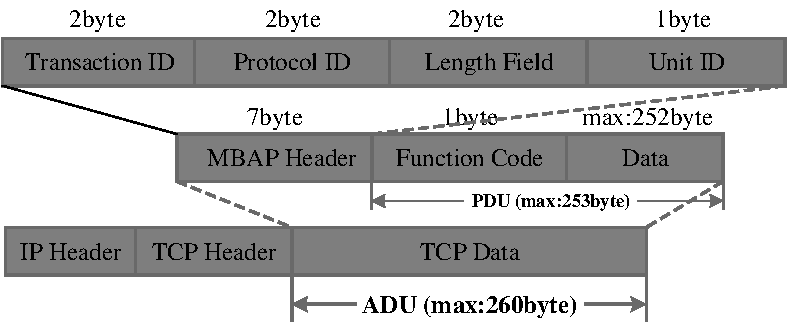
\includegraphics[width=3.2in]{FIGURE_LV/FigModbusFormat.pdf}
	\caption{Message format of Modbus-TCP}
	\label{FigModbusFormat}
\end{figure}

\subsubsection{EtherCAT}
EtherCAT offers high real-time performance and provides a master-slave communication mode among the industry devices. A typical EtherCAT network consists of one master and several slaves. The master generates datagrams and sends them to the loop network. These datagrams are reflected at the end of each network segment and sent back to the master. We test EtherCAT to prove the versatility of our method.

\subsection{Training Data}
Training data in deep learning significantly influence model training. Thus, we accurately collect and preprocess the training data. In the experiment, training data about the two industrial control protocols is collected separately.

\subsubsection{Modbus-TCP}
We use the Pymodbus \cite{Pymodbus}, a python package that implements the Modbus protocol, to generate the training data frames. Through it, we can quickly generate enough different types of data frames conveniently. Specifically, 300,000 pieces of data, including various type, are used as the training data. The data set is divided into a training set, a verification set, and a test set according to the proportion of 10-fold cross-validation.

\subsubsection{EtherCAT}
In order to capture the EtherCAT communication data, we prepare an EtherCAT based ICS. The master station is a Beckhoff \cite{Beckhoff} industrial PC, and the slave station includes EK1100 \cite{EK1100},  EL1004 \cite{EL1004} and EL2004 \cite{EL2004}. ET2000 \cite{ET2000} is used as the online Listener between the master and the slaves. The Wireshark \cite{Wireshark}, running on a computer, can fetch and display the massive communication data messages from the listener. After processing, these messages will serve as the training data for the EtherCAT protocol.
\begin{figure}[htbp]
\centering
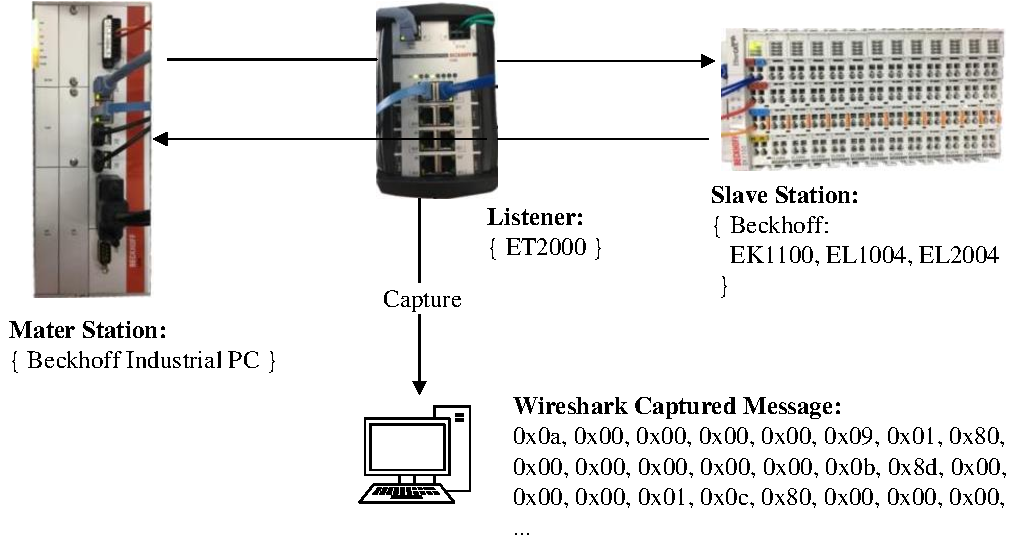
\includegraphics[width=3.3in]{FIGURE_LV/FIGURE_ETHERCAT.pdf}
\caption{EtherCAT enviroment}
\label{FIGURE_DGD}
\end{figure}

\subsection{Evaluation Setup}
\subsubsection{Experimental Environment}
We adopted Tensorflow, one of the popular deep learning framework, to implement the model architecture. To improve the training efficiency, we train the model on a Windows machine with 8 processors (Intel (R) Core (TM) i7-6700K CPU@4.00GHz) 16.0GB memory (RAM) Nvidia GeForce GTX 1080 Ti (11GB). When launching an attack, the simulators run on another machine with 4 processors (Intel (R) Core (TM) i5-5300U CPU@2.30GHz) 8.00GB memory (RAM).
\subsubsection{Model Training Setting}
As for the parameter setting, we initialize all weights from zero-centered Normal distribution with a standard deviation of 0.02. The mini-batch size is set to 256 in all models. The learning rate is set to 0.0002 in the Adam optimizer. As to the Leaky ReLU function in the discriminator model, the slope of the leak is set to 0.2. We train the models for 100 epochs and save the generator model for every ten epochs to get plentiful test cases.

\subsection{Experiment Results}
In this section, we show the experimental results in three aspects. We first present the bugs that occurred in the process of fuzzing the Modbus implementations. Then we reveal statistical results and its analysis. Lastly, to show protocol independence of our methodology in ICP’s fuzz testing, we apply it to test the EtherCAT protocol.
\subsubsection{Exception Founded}
We send the generated data frames to the aforementioned Modbus implementations which serve as Modbus slave stations. A total of 270,000 test cases generated was sent to each Modbus implementations. The effect is exciting that we successfully triggered bugs. The following describes these bugs in detail.

Much abnormal information is displayed at the console of the simulation software when the Modbus Rssim is attacked by the generated data frames. For a while, it goes crash. In detail, the software pop-ups windows prompt box after we sent about 3500 data frames, indicating that the program has crashed. We send data frames range from 3450th to 3500th to the other two simulation softwares, Modbus Slave and xMasterSlave; no abnormality occurs. This comparison shows that Modbus Rssim has some errors in the emulating Modbus-TCP protocol.

Another exception worth discussing is ``Station ID xx off-line, no response sent" in Modbus Slave. The log indicates that “Station ID 32 off-line, no response sent” after sending about 6540 data frames. But we observe that the station 32 is still online. This phenomenon makes us believe that there is an implementation flaw with the slave state judgment of Modbus Slave.

In fuzz testing the xMasterSlave, we find that the software automatically closes the window itself at times. Through the analysis of the system log, we conclude that memory overflow is the cause of the software crash, which suggests that the programmer may not consider the exception of populating with data boundary values when implementing the simulator. 

In further attacks of fuzz testing the three simulation softwares and the real environment, anomalies such as ``Using Abnormal Function Code", ``Data length Unmatched", ``Integer Overflow" and ``Abnormal Address" occur on a regular basis. We record the test cases that cause these abnormalities. All the abnormal feedbacks from the three softwares and slaves in the real environment are counted for further analysis. Other anomalies, such as ``File not Found" and ``Debugger Memory Overflow" and so on, are found only once or twice and thus are not discussed in detail.

\subsubsection{Statistical Analysis And Results}
In the study, we choose the widely used GPF \cite{demott2007revolutionizing}, GAN-based model and LSTM-based seq2seq mode as fuzzers in the control group. The systems to be tested are 3 Modbus simulation softwares, namely Modbus Slave, xMasterSlave, Pymodbus and Modbus RSSIM, and the real Modbus network environment we put up. In order to better evaluate the overall effect of the model on the protocol, we combined the experimental results of the four systems. The weights of the data obtained in these four experiments are 20\%, 20\%, 20\%, 40\% in the holistic data.

After fuzzers in the experimental group and control group are fully trained, fuzzing test is conducted by sending generated test cases through the TCP/502 port.

According to the three evaluation indicators mentioned above, we evaluate the effectiveness and efficiency of our fuzzing framework BLSTM-DCNNFuzz. Details are as follows.

\quad \textit{\textbf{a. TCRR.}}

GPF is compared with the other three fuzzing models based on depth learning, and the experimental results about $TCRR$ are shown in Fig. \ref{FIGURE_TCRR}. The horizontal line represents the performance of GPF on the systems. Due to not involving the learning process, there is no changing trend of GPF.

From the perspective of the four experiments, the performance of the TCRR indicators is: GPF $\approx$ LSTM-based model $\textless$ GAN-based model $\textless$ BLSTM-DCNNFuzz. After training more than 30 epochs, the TCRR rates of generative adversarial algorithms obviously exceed GPF algorithm, and the rising trend of rate slows down significantly after 60 epochs. The average TCRR rate of the GPF is 58. 5\%, and the TCRRs rate for generative adversarial algorithms is 75\% to 90\%. The final TCRR rate of the LSTM-based model algorithm is significantly lower than the other two groups for deep learning, which may be caused by the inability to learn the spatial characteristics of the data effectively. The function codes and parameters range of the protocol message are limited, which increases the possibility of abnormal exception in the random generation. For the generative adversarial algorithms from 50 to 100 epochs, the average TCRR rate of BLSTM-DCNNFuzz is approximately 8\% higher than GAN, which indicates that BLSTM-DCNNFuzz is more applicable to test cases generation for ICPs indirectly.
\begin{figure}[htbp]
	\centering
	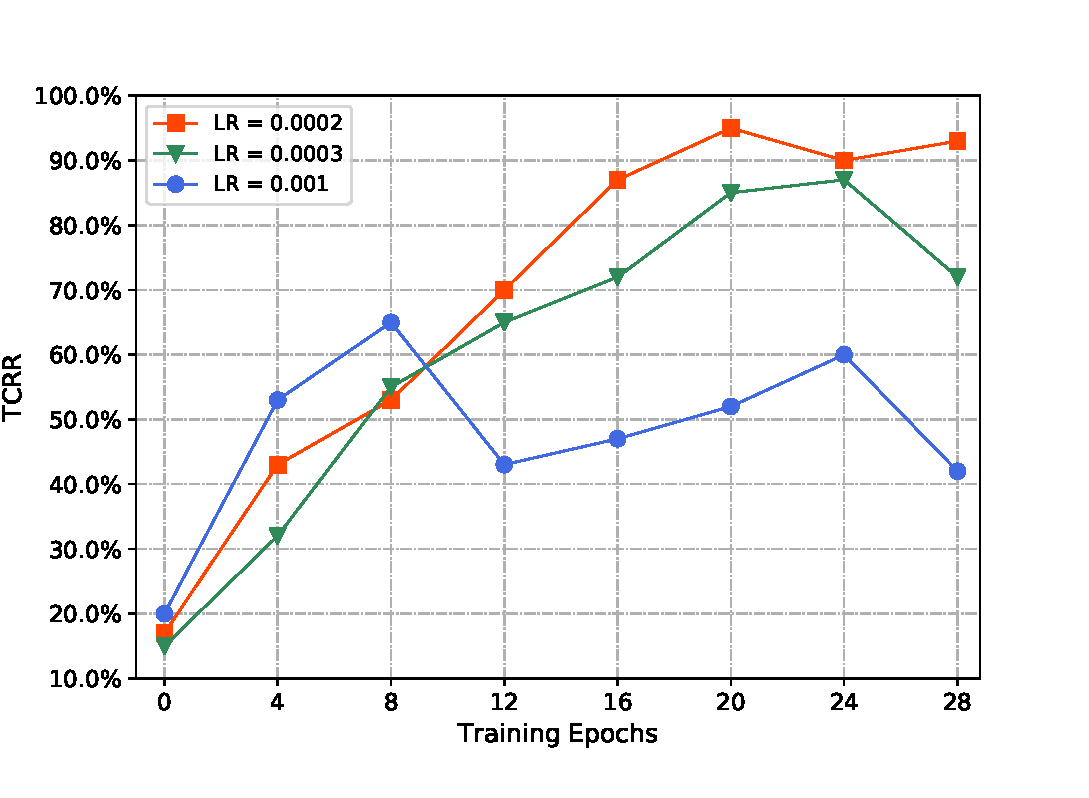
\includegraphics[width=3.36in]{FIGURE_LV/FIGURE_TCRR.pdf}
	\caption{TCRR changes with the training epochs}
	\label{FIGURE_TCRR}
\end{figure}


\quad \textit{\textbf{b. BTE.}}

When testing the Modbus implementations, we recorded triggered bugs and triggered frequency. The fuzzing test results of the four models are as follows: Table \uppercase\expandafter{\romannumeral2}. The result comparison shows our proposed methodology can trigger more vulnerabilities in higher frequency than other models, which shows the testing efficiency of BLSTM-DCNNFuzz.
\begin{table}[htbp]
	\caption{Experimental Data Comparison}
	\label{table_example}
	\centering
	\begin{tabular}{m{70pt}<{\centering}  p{30pt}<{\centering} p{30pt}<{\centering}  p{32pt}<{\centering}  p{30pt}<{\centering}}% p{40pt}p{30pt}p{40pt}p{50pt}p{40pt}
		\toprule
		\bfseries Test Model &  \bfseries Case Amount &  \bfseries Test time/h &\bfseries Bugs triggered  &\bfseries BTE Score\\
		\midrule
		BLSTM-DCNNFuzz & 18,000 & 16 & 674 & 1.37\\
		GAN-based model & 38,785 & 3 & 101 & 0.98\\
		LSTM-based model & 128,711 &  9 & 283 & 0.86\\
		GPF				 & 120,000 & 28 & 49   & 0.15 \\
		\bottomrule
	\end{tabular}
\end{table}

The concrete manifestation of BLSTM-DCNNFuzz is shown in Table \uppercase\expandafter{\romannumeral3}. 
\begin{table}[htbp]
	\caption{Triggered Bugs and Triggered Frequency of BLSTM-DCNNFuzz}
	\label{table_example}
	\centering
	\begin{tabular}{lccc}
		\toprule
		\bfseries Triggered bugs &  \bfseries Frequency (Times) & \bfseries Sent number\\
		\midrule
		Slave crash & 57 & 30,000\\
		Station ID xx off-line & 177 & 30,000 \\
		Using Abnormal Function Code & 248 & 30,000 \\
		Automatically closes the window & 73 & 30,000\\
		Data length Unmatched & 26 & 30,000 \\
		Abnormal Address & 83 & 30,000 \\
		Integer Overflow & 5 & 30,000 \\
		File not found & 3 & 30,000\\
		Debugger memory overflow & 2 & 30,000 \\
		\bottomrule
	\end{tabular}
\end{table}

\quad \textit{\textbf{c. DGD.}}
The message categories learned by GPF is constant and the coverages of different GPF are different, so it is not discussed here. The testing depth has increased as illustrated in Fig.\ref{FIGURE_TCRR} at the expense of reducing the code coverage of fuzzing test. Therefore, we need to maintain high test case diversity on the premise of attaining high TCRR rates. A total of 13 types of Modbus data frames are prepared in the original training data. When the training epochs is 10, the diversity of 3 models maintains the best. After training, some message categories are generally lost, as presented in Fig. \ref{FIGURE_DGD}. BLSTM-DCNNFuzz and LSTM-based model have good performance on maintaining basically the test case diversity, which illustrates the two models can learn the time-step dimension of protocol messages. And owing to BLSTM-DCNNFuzz containing two sub-networks for the forward and backward sequence context respectively in the BLSTM layer of BLSTM-DCNNFuzz, it is able to exploit information from both the past and the future, which performs better than LSTM-based model. Usually, the richer the data type, the higher code coverage we are likely to reach, and the stronger ability a model has to detect anomalies. Thus as presented in Table \uppercase\expandafter{\romannumeral3}, our trained model can effectively detect kinds of bugs.

\begin{figure}[htbp]
	\centering
	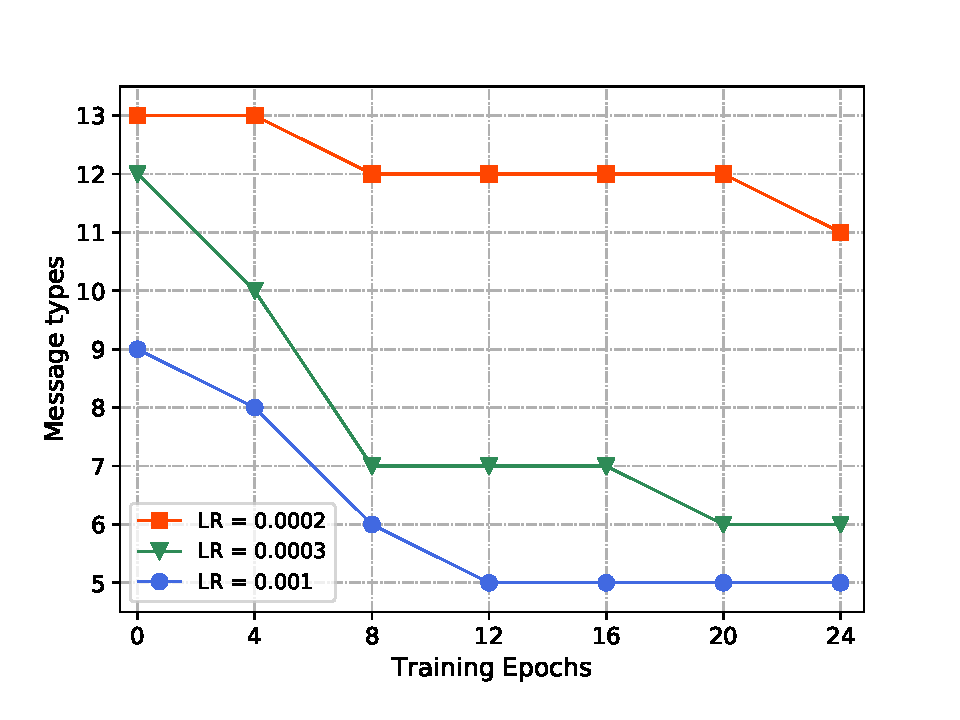
\includegraphics[width=3.3in]{FIGURE_LV/FIGURE_DGD.pdf}
	\caption{Data diversity retention}
	\label{FIGURE_DGD}
\end{figure}

\subsubsection{Applying The Method to Another ICP-EtherCAT}
To demonstrate our methodology is not just akin to a particular ICP, we apply BLSTM-DCNNFuzz to test EtherCAT, another widely used ICP. We retrain the model with captured EtherCAT data frames. With the newly trained model, massive test cases are generated expediently to detect the potential vulnerabilities of the EtherCAT protocol. The following presents the details.

\quad \textit{\textbf{a. Communication details of EtherCAT.}} EtherCAT uses a dedicated Ethernet data frame type definition to transport EtherCAT packets of Ethernet data frames. The master station initiates the communication process and controls the working status of the slave stations via process data communication. The EtherCAT slave stations extract the control information and commands from the protocol messages sent by the master station, and insert the relevant information and the collected data of the local industrial field device associated with itself. Then this Ethernet data message is transferred to the next EtherCAT slave stations. The operation repeats until all slave stations are traversed. 

\quad  \textit{\textbf{b. Detected potential vulnerabilities.}} As shown in Table \uppercase\expandafter{\romannumeral4}, we detected these potential vulnerabilities, including man-in-the-middle (MITM), MAC address spoofing, slave address attack, packet injection, working counter (WKC) attack and so on. In the experiment, we send the generated data messages $S_i$ to the slave stations and record the corresponding received message $R_i$. We get massive message pairs $<S_i, R_i>$. According to the abnormal protocol characterization above, we analyzed and compared the specified field values and obtained the following statistical results. Experiments on the EtherCAT protocol prove that our method has great versatility.
\begin{table}[htbp]
\caption{Potential Vulnerabilities and occurrences times in EtherCAT}
\label{table_EtherCAT}
\centering
\begin{tabular}{lcc}
    \toprule
    \makecell[tl]{\bfseries Potential Vulnerabilities} &  {\bfseries Occurrences times} & {\bfseries Sent Number} \\
    \midrule
    \makecell[tl]{Packet Injection Attack}  & {178 times} & 30,000 \\
    \makecell[tl]{Man In The Middle Attack} & {26 times} & 30,000 \\
    \makecell[tl]{Working Counter Attack}   & {209 times } & 30,000 \\
    \makecell[tl]{MAC Address Spoofing}  & {41 times} & 30,000 \\
    \makecell[tl]{Slave Address Attack}  & {13 times} & 30,000 \\
    \makecell[tl]{Unknown Attack}  & {597 times} & 30,000 \\
    \bottomrule
\end{tabular}
\end{table}




\section{Conclusions and Future works}
In this study, we propose an effective fuzzing methodology based on DCGAN to generate fake but plausible fuzzing data about ICPs. This methodology utilizes CNN to learn the spatial structure and distribution of real-world messages and generate similar data frames without knowing the detailed protocol specification. Allowing the convolution neural networks to learn message formats can save human effort and reduce time. In this manner, when testing other network protocols, we do not need to understand their specifications, which is convenient. We ultimately evaluate this method by fuzzing two safety-critical ICPs, including Modbus-TCP and EtherCAT. The results indicate that the proposed method has application potential to test a series of ICPs.

In future studies, we expect to create a more intelligent and more automated network protocol fuzzing system deployed to embedded devices. The system can apply the manner of online learning to learn protocol specifications or message formats of different protocols automatically. Considering the current situation, we intend to perform the study in the following aspects. First, we want to do a further exploration of other architectures to enhance our approach. Second, we will use our method to test other stateful ICPs, such as Profibus, Powerlink and future TSN. These protocols constitute an important part of most current ICPs. Finally, we intend to integrate each excellent architecture and processing module to form a hybrid model and a complete software system, which can deal with most network protocols, including stateful protocols and non-stateful protocols.

\nocite{*}
\bibliographystyle{IEEEtran}
\bibliography{Reference}

\end{document}
